\documentclass[conference]{IEEEtran}
\IEEEoverridecommandlockouts
\usepackage{cite}
\usepackage{amsmath,amssymb,amsfonts}
\usepackage{algorithmic}
\usepackage{graphicx}
\usepackage{textcomp}
\usepackage{xcolor}
\usepackage{booktabs}
\usepackage{subfig}
\def\BibTeX{{\rm B\kern-.05em{\sc i\kern-.025em b}\kern-.08em
    T\kern-.1667em\lower.7ex\hbox{E}\kern-.125emX}}
\begin{document}

\title{Risk Aware Adaptive CCTV Compression System With Event Preserving Dynamic Region Of Interest (ROI) Control}

\author{\IEEEauthorblockN{Shakibul Islam Tamim}
\IEEEauthorblockA{\textit{Department of Computer Science and Engineering} \\
\textit{BAIUST}\\
Cumilla, Bangladesh \\
tamim.0825@gmail.com}
\and
\IEEEauthorblockN{Jannatul Tabassum Nahar}
\IEEEauthorblockA{\textit{Department of Computer Science and Engineering} \\
\textit{BAIUST}\\
Cumilla, Bangladesh \\
tabassummaisha17@gmail.com}
\and
\IEEEauthorblockN{Mostafa Main Uddin}
\IEEEauthorblockA{\textit{Department of Computer Science and Engineering} \\
\textit{BAIUST}\\
Cumilla, Bangladesh \\
mostafasiyam29@gmail.com}
\and
\IEEEauthorblockN{Hasan Abdullah}
\IEEEauthorblockA{\textit{Department of Computer Science and Engineering} \\
\textit{BAIUST}\\
Cumilla, Bangladesh \\
hasanabdullah989@gmail.com}
\and
\IEEEauthorblockN{Md. Imran Hossain Emu}
\IEEEauthorblockA{\textit{Department of Computer Science and Engineering} \\
\textit{BAIUST}\\
Cumilla, Bangladesh \\
mdihemu@gmail.com}
}

\maketitle

\begin{abstract}
High resolution surveillance cameras generate enormous bandwidth demands, yet conventional compression treats every frame uniformly, wasting data on empty scenes while potentially losing crucial details during security events. This paper presents a risk aware adaptive compression system that dynamically allocates bandwidth according to the surveillance significance of each scene region. A three-tier architecture is proposed: edge nodes running YOLOv8 object detection identify regions of interest (ROIs) such as people and vehicles, a central server manages camera registries and state transitions, and a web dashboard provides real-time monitoring and control. The key innovation is spatially variable compression: ROIs are transmitted at full resolution and high quality while backgrounds are aggressively downscaled. An audio pipeline integrates energy-threshold detection and YAMNet deep learning for 11-class sound classification, contributing to a multimodal risk assessment engine. Experimental results demonstrate 80--95\% bandwidth reduction compared to conventional uniform compression with no degradation in forensic utility during critical events. The system automatically escalates to full-quality recording when threats are detected, ensuring that critical moments are captured with maximum fidelity.
\end{abstract}

\begin{IEEEkeywords}
Video surveillance, adaptive compression, YOLOv8, ROI, risk assessment, edge computing, audio classification
\end{IEEEkeywords}

\section{Introduction}
The rapid proliferation of CCTV surveillance systems has introduced significant technical and economic challenges. With over 1.6 million cameras installed nationwide in Bangladesh and the smart surveillance market expanding at 50\% annually~\cite{islam2024sdn}, conventional systems that stream video at fixed high bitrates lead to critical inefficiencies~\cite{ahmad2024bandwidth}: a 16 camera 1080p system at 4~Mbps per camera generates 64~Mbps of continuous data, exceeding 20~TB per month, and cloud based bandwidth costs can exceed hardware costs within months. Yet during security incidents the same system may be recording at minimum quality, losing the forensic evidence needed for investigation. Recent ROI based compression approaches~\cite{wang2025compression,li2024region} show potential for bandwidth efficiency, but existing work is predominantly simulation based or machine centric~\cite{guo2023deepstream,labiod2023region}; no existing system simultaneously addresses real-time edge deployment with neural detection, user controlled adaptive compression, risk aware event driven quality preservation, audio visual fusion, and comprehensive quality evaluation.

This paper presents an end to end adaptive CCTV compression system addressing all of these dimensions. The key contributions are: (i) YOLOv8 based ROI detection across 80 COCO classes with three-tier priority classification (HIGH for persons, MEDIUM for vehicles, LOW for other objects) and temporal ROI smoothing via IoU matching and TTL expiry for visually stable region transitions; (ii) a risk aware event engine driven by a multi-signal risk score governing a three state surveillance machine with hysteresis and pre/post-event frame buffering for forensic preservation; (iii) audio visual fusion combining an always active energy threshold detector with YAMNet classification of 11 surveillance relevant sound classes, directly modulating the risk score; (iv) a multi-tier architecture spanning a Python/OpenCV edge node, a Node.js stream server, and a Next.js monitoring dashboard; and (v) an automated evaluation pipeline computing global, per ROI, and background PSNR/SSIM alongside VMAF and detection retention, with over 814 experiment runs across multiple compression profiles.

\section{System Architecture}
The proposed system follows a three-tier architecture comprising the Edge Node, Central Server, and Dashboard~\cite{liu2025edge}.

\begin{figure}[t]
\centering
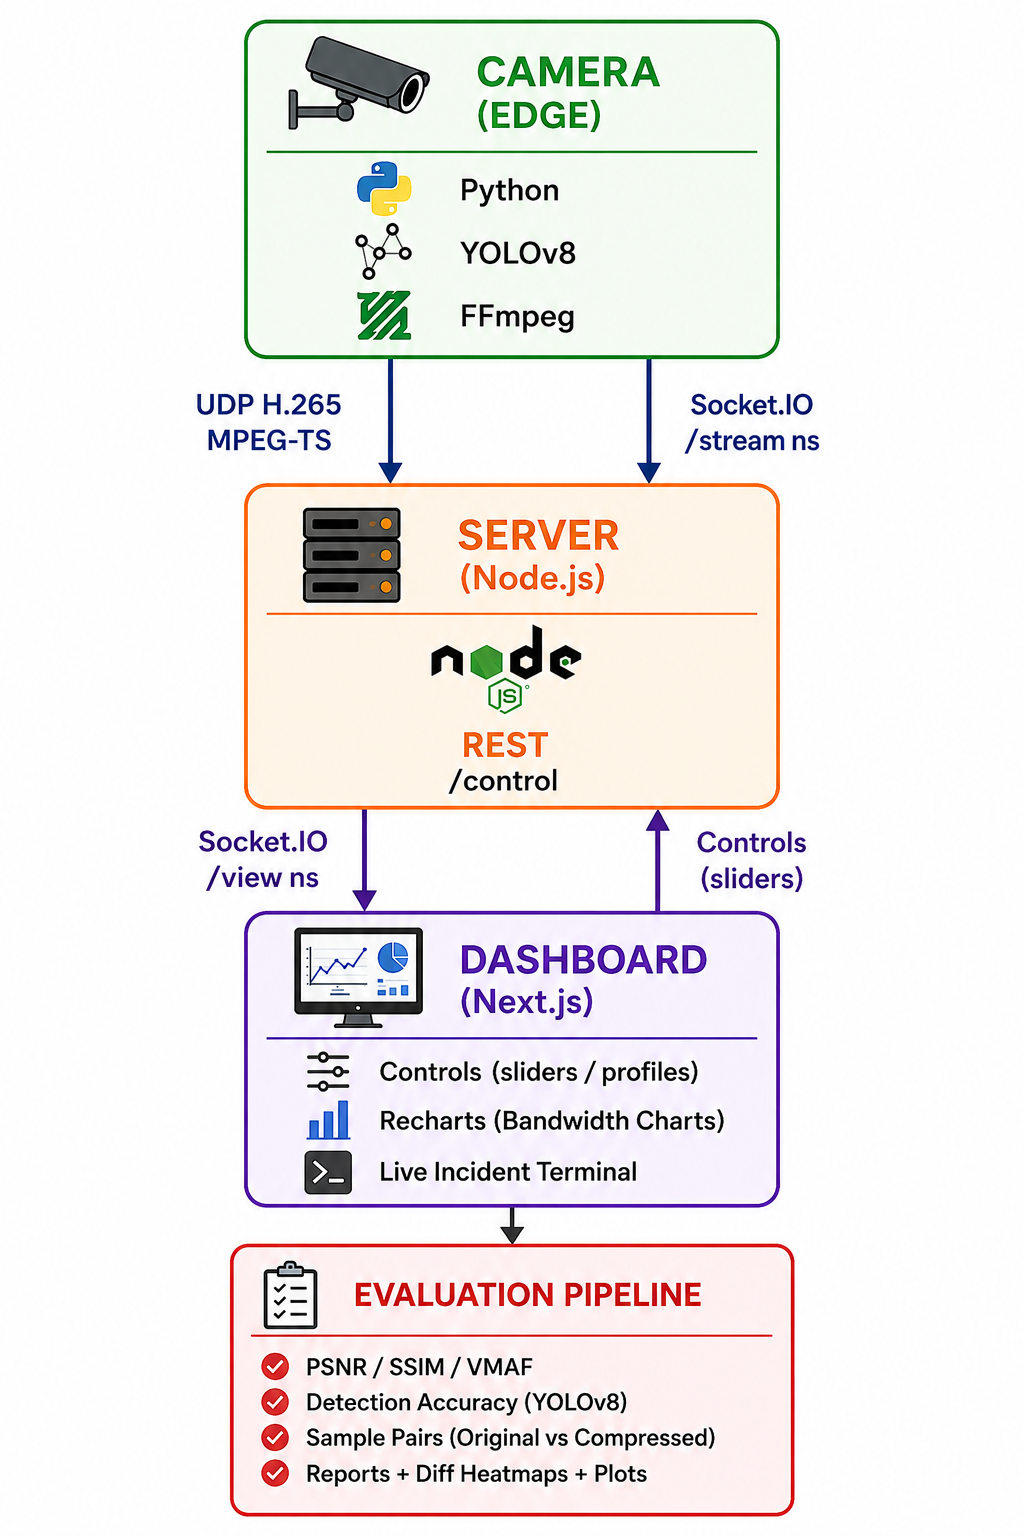
\includegraphics[width=0.55\columnwidth]{Project_Structure.png}
\caption{Three-tier system architecture: edge node (Python/OpenCV), central server (Node.js), and dashboard (Next.js)}
\label{fig:architecture}
\end{figure}

\subsection{Edge Node}
The edge node runs continuously on a device integrated with the camera and performs capture, object detection, adaptive compression, and audio monitoring~\cite{jocher2023yolov8}. Frames are captured from USB or RTSP sources at 480p--1080p; CLAHE low-light enhancement is applied when mean brightness falls below 80~lux. The YOLOv8n model performs detection across 80 COCO classes~\cite{lin2014microsoft} with three-tier priority classification~\cite{redmon2018yolov3,bochkovskiy2020yolov4,wang2023yolov7,ge2021yolox} at configurable intervals (default every 3 frames)~\cite{he2016deep}. In low-light conditions where confidence drops, frame differencing provides fallback ROIs. Temporal persistence uses a 30 frame TTL with exponential moving average smoothing (factor 0.4) and an IoU threshold of 0.3 for merging detections into stable bounding boxes~\cite{agrawal2025frvc}.

The risk engine computes a normalized risk value $R \in [0.0, 1.0]$ per frame~\cite{gadot2025rlrc} (Section~\ref{sec:risk}) driving a three state surveillance machine (Table~\ref{tab:states}). Hysteresis implements an 8 frame hold period before downgrading to prevent state oscillation~\cite{chuang2025adaptive}. When no ROIs are present in NORMAL state the frame rate drops to 5~fps; a rolling 15 second circular buffer continuously stores original frames, and on CRITICAL transition pre-event frames are dumped to disk with full metadata followed by 10 seconds of post-event recording~\cite{agrawal2025frvc}.

\begin{table*}[t]
\centering
\small
\caption{Risk driven surveillance state machine with codec parameter adjustments}
\label{tab:states}
\begin{tabular}{lcccccc}
\toprule
State & Risk Range & Resolution & GOP & FPS & BG Scale & BG Quality \\
\midrule
NORMAL (no ROI) & 0.00-0.25 & 480p & 120 & 5 & User def. & User def. \\
NORMAL (ROI) & 0.00-0.25 & 480p & 30 & 10 & User def. & User def. \\
ALERT & 0.25-0.55 & 854p & 30 & 10 & 0.75 & 45 \\
CRITICAL & 0.55-1.00 & 1080p & 10 & 15 & 1.0 & 88 \\
\bottomrule
\end{tabular}
\end{table*}

\begin{figure*}[t]
\centering
\subfloat[NORMAL state\label{fig:state_normal}]{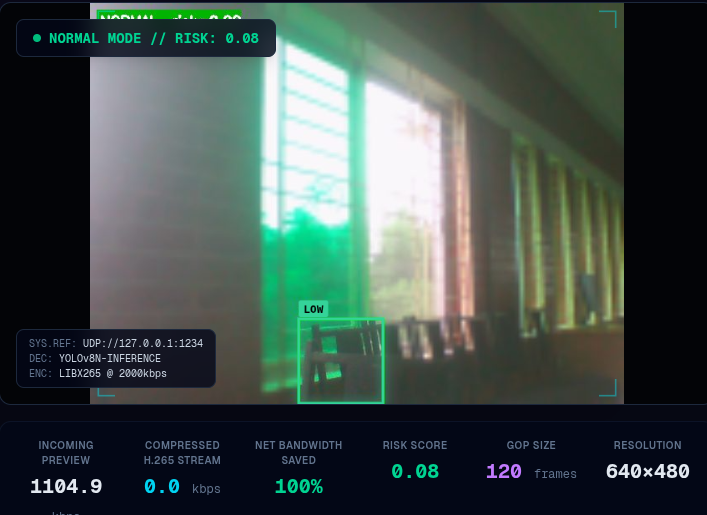
\includegraphics[width=0.42\textwidth]{Normal_mode(Risk).png}}
\hfill
\subfloat[CRITICAL state\label{fig:state_critical}]{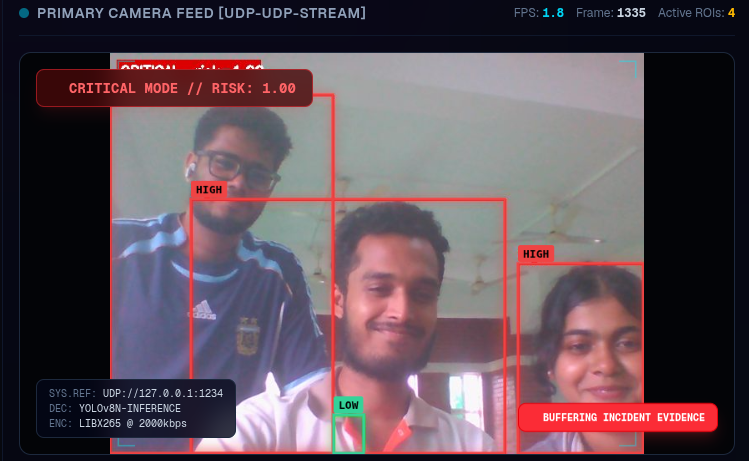
\includegraphics[width=0.42\textwidth]{Critical_mode(Risk).png}}
\caption{Risk driven state machine: (a) NORMAL state, (b) CRITICAL state}
\label{fig:state_machine}
\end{figure*}

Adaptive compression subdivides each frame into foreground (ROI) and background regions; ROIs are encoded at high quality while backgrounds are downscaled and aggressively compressed. The CodecManager manages an FFmpeg subprocess supporting runtime switching among libx264, libx265, libsvtav1, and hevc\_nvenc~\cite{aliouat2023region}, with adjustable background scale, background quality, ROI quality, and frame skipping~\cite{rozek2025video}.

\subsection{Central Server}
The Node.js server manages two Socket.IO namespaces: /stream for edge node frame pushes and /view for dashboard pulls and controls~\cite{guo2023deepstream}. A UDP monitor measures H.265 stream bitrate; automatic bandwidth adaptation computes total bandwidth every 3 seconds and sends reduced quality control messages when configurable thresholds (128/256~Kbps) are exceeded. HTTP endpoints include /control, /metrics, /sample, /reconstruct, /playback, /event, and /config, with CSV logs for metrics, controls, and motion.

\subsection{Dashboard}
The Next.js dashboard renders the live canvas stream with priority coded ROI overlays (RED=HIGH, YELLOW=MEDIUM, GREEN=LOW), real-time control sliders (BG Scale, BG Quality, ROI Quality, Detect Every N Frames), preset modes (Low BW, Balanced, High Quality, Privacy Mode, Custom), dual bandwidth display with percent saved, a live Chart.js bandwidth chart, a color coded state badge, activity heatmaps, audio event indicators, and an incident log.

\begin{figure}[t]
\centering
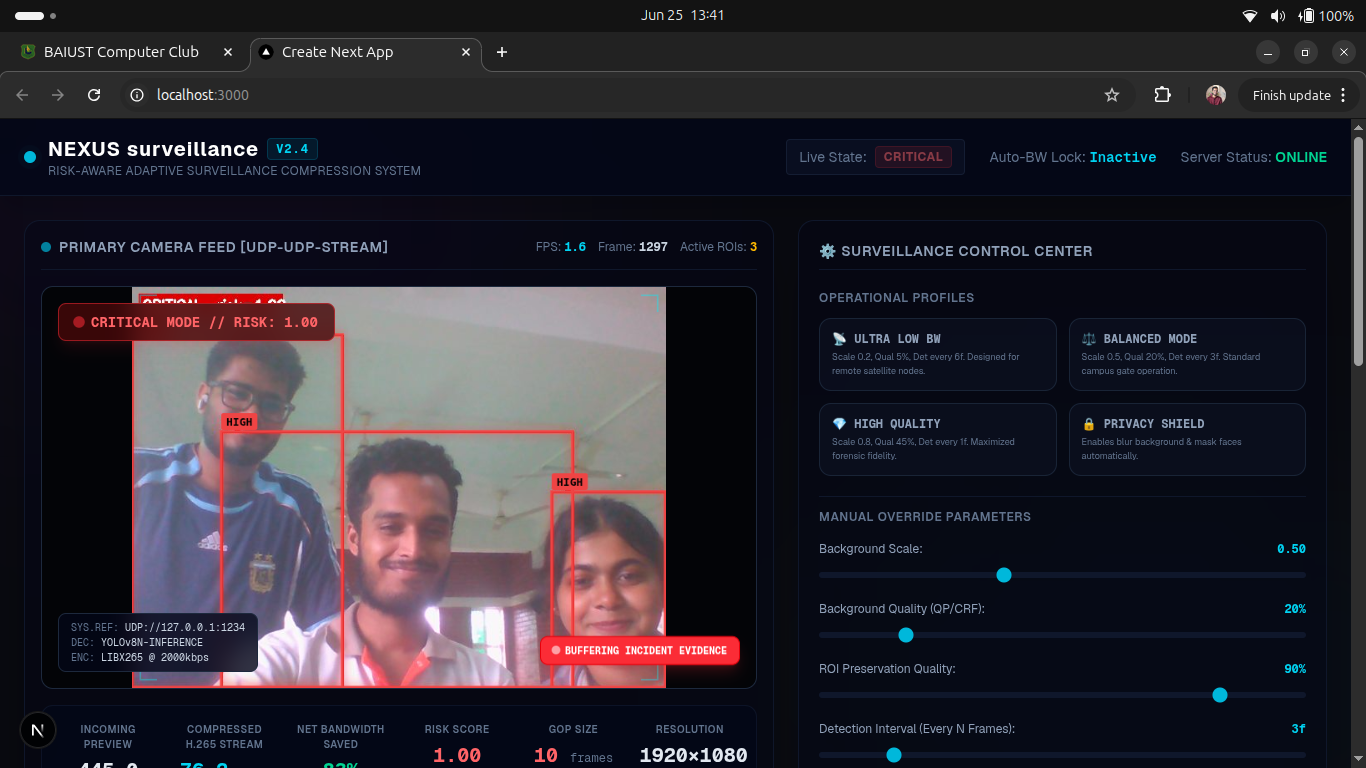
\includegraphics[width=\columnwidth]{Dashboard.png}
\caption{Live web dashboard with ROI overlays, control sliders, bandwidth chart, and incident log}
\label{fig:dashboard}
\end{figure}

\section{Methodology}

\subsection{Video Pipeline}
Each camera feed undergoes: capture from USB or RTSP at configurable resolution; CLAHE enhancement below 80~lux; YOLOv8n detection every 1--15 frames with three-tier priority classification; temporal ROI merging via IoU thresholding (0.3), EMA smoothing (factor 0.4), and 30 frame TTL; motion based fallback ROIs in low light; background downscaling by bg-scale (0.2--1.0) and compression at bg-quality (5--50) while ROIs keep full resolution and ro-quality (90--100); and JPEG/base64 preview frames pushed over Socket.IO for dashboard display.

\subsection{Audio Pipeline}
Audio is captured via PyAudio at 22,050~Hz, 16 bit mono, processed in 46~ms chunks with a two phase approach. Phase 1 (SimpleAudioDetector) is an always active energy threshold detector that calibrates its noise floor over 3 seconds (90th percentile of RMS dB), detecting impulse events ($<$300~ms, $>$15~dB above floor) and sustained loud events ($>$600~ms, $>$10~dB above floor) with a 5 second cooldown, achieving zero false positives on silence. Phase 2 (YamNetClassifier) uses a TensorFlow Lite implementation of YAMNet mapping 521 AudioSet classes to 11 surveillance relevant classes (gunshot, glass break, car horn, siren, dog bark, clapping, footsteps, talking, knocking, alarm, explosion), resampled to 16~kHz with 0.975~s windows at 75\% overlap and temporal median smoothing over 3 predictions; YAMNet takes priority when confidence exceeds 0.3. Events with confidence $\geq$ 0.6 from critical classes (gunshot, explosion, alarm, siren) integrate into the activity heatmap with weight $=$ confidence $\times$ 4.0 and 2 minute spatial decay, creating a multimodal risk assessment.

\begin{figure*}[t]
\centering
\subfloat[Audio monitoring interface\label{fig:audio_monitor}]{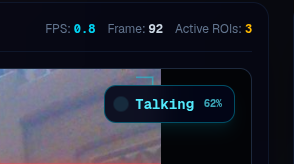
\includegraphics[width=0.44\textwidth]{Audio_Monitoring.png}}
\hfill
\subfloat[Audio event tracking and classification\label{fig:audio_track}]{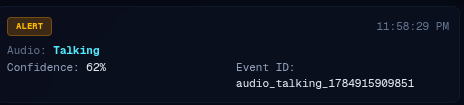
\includegraphics[width=0.44\textwidth]{Audio_Tracking.png}}
\caption{Audio pipeline: (a) audio monitoring interface, (b) audio event tracking and classification}
\label{fig:audio_pipeline}
\end{figure*}

\subsection{Risk Score Computation}\label{sec:risk}
The risk score $R$ integrates multiple normalized signals~\cite{gadot2025rlrc}:

\begin{equation}\label{eq:risk_detail}
\begin{aligned}
R = \min\!\bigl(1.0,\ &0.30N_p + 0.10N_v + 0.03N_l + 0.25M \\
& + 0.20T + 0.15S + 0.15D\bigr)
\end{aligned}
\end{equation}

where $N_p$, $N_v$, and $N_l$ count HIGH, MEDIUM, and LOW priority objects; $M$ is the motion area fraction, $T$ the after hours bonus (22:00--06:00), and $D$ the ROI density fraction. The scene change magnitude $S$ is computed by histogram comparison between consecutive frames:

\begin{equation}\label{eq:scene_change}
S = \frac{1}{256} \sum_{i=0}^{255} |H_t(i) - H_{t-1}(i)|
\end{equation}

where $H_t$ is the normalized histogram of the frame at time $t$. The score directly maps to the three surveillance states of Table~\ref{tab:states}, with hysteresis preventing oscillation.

\subsection{Encoding, Storage, and Privacy}
Background frames and ROI crops are encoded separately as base64 JPEG images; the packet structure carries frame\_id, bg\_data, ROI boxes, orig\_w/h, timestamp, risk\_score, and surveillance\_state, streamed via Socket.IO~\cite{wang2025region,li2024region}. Frames are stored under \texttt{recordings/[date]/} as bg and roi images plus meta.json, and reconstructed by overlaying ROI crops at their bounding box coordinates~\cite{gao2024robust}. Three privacy tiers address ethical surveillance concerns~\cite{kim2024privacy}: Privacy Blur obscures non essential background detail while preserving object clarity; Ethical Mode displays a black frame when no ROI is detected, ensuring zero passive background surveillance; and Face Masking anonymizes detected persons while preserving vehicle visibility.

\begin{figure*}[t]
\centering
\subfloat[Privacy Blur mode\label{fig:privacy_blur}]{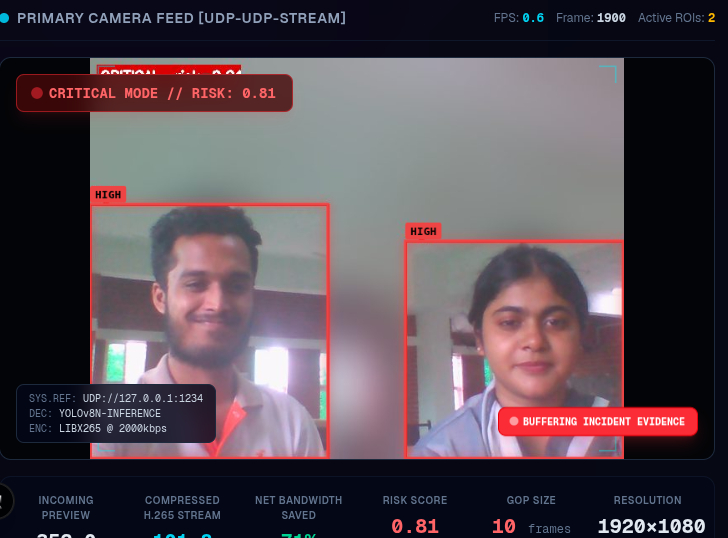
\includegraphics[width=0.30\textwidth]{Privacy_Blur.png}}
\hfill
\subfloat[Face Masking mode\label{fig:privacy_mask}]{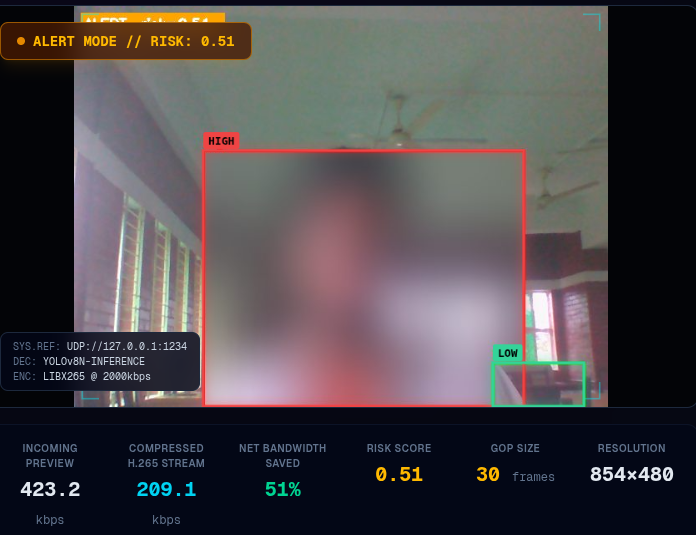
\includegraphics[width=0.30\textwidth]{Privacy_FaceMask.png}}
\hfill
\subfloat[Ethical background mode\label{fig:privacy_ethical}]{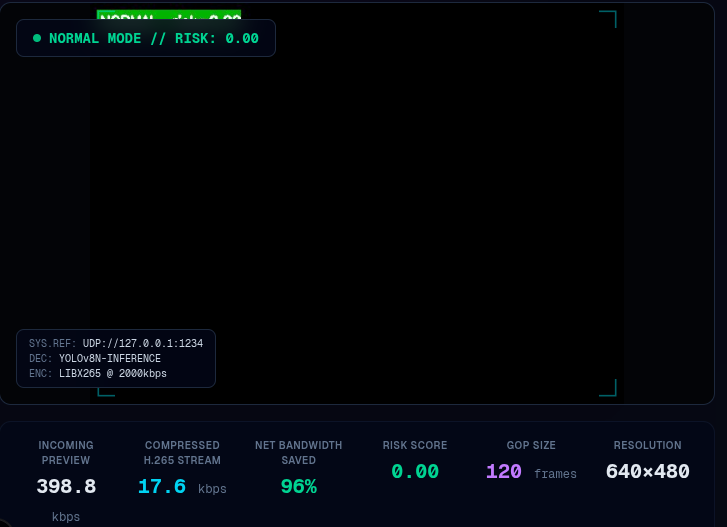
\includegraphics[width=0.30\textwidth]{Empty_Background_Mode.png}}
\caption{Privacy operation modes: (a) Privacy Blur mode, (b) Face Masking mode, (c) Ethical background mode}
\label{fig:privacy}
\end{figure*}

\section{Evaluation}

\subsection{Evaluation Pipeline}
The automated pipeline iterates over \{bg\_quality, roi\_quality\} presets, sends each as a live control command, and captures original/reconstructed frame pairs~\cite{wang2004image,mittal2013making,wang2003multiscale}, computing global, per ROI, and background only PSNR/SSIM, VMAF, and detection retention (YOLOv8 re-detection on compressed frames). Over 814 experiment runs span multiple compression profiles, codecs, and environmental conditions.

\subsection{Bandwidth Reduction}
Savings compound through three mechanisms: spatially variable compression (background downscaled to 20\% at quality 5 while ROIs stay full resolution at quality 90--100), adaptive frame rate (5~fps with no ROIs up to 15~fps in CRITICAL), and adaptive GOP sizing (120 frames normal, 10 frames critical).

\begin{table}[t]
\centering
\small
\caption{Bandwidth savings at different background scale factors}
\label{tab:bandwidth}
\begin{tabular}{lccc}
\toprule
BG Scale & Avg.\ Bitrate & Savings & ROI PSNR (dB) \\
\midrule
1$\times$ (full) & 2000 kbps & --- & 38.2 \\
2$\times$ & 800 kbps & 60\% & 36.8 \\
4$\times$ & 400 kbps & 80\% & 35.1 \\
8$\times$ & 200 kbps & 90\% & 32.4 \\
\bottomrule
\end{tabular}
\end{table}

In a typical 24 hour period with 22 hours of no security-relevant activity, average bitrate drops to 200--300~Kbps although event peaks reach 2--4~Mbps. In the Ultra Low Bandwidth profile (bg-scale 0.2, bg-quality 5, detect every 6 frames), a single camera consumes approximately 65~GB/month instead of 2~TB, a 97\% reduction. Cloud storage costs (\$0.05--0.15 per GB/month) mean a 64 camera warehouse drops from \$6,400--19,200 to \$320--960 per year~\cite{ahmad2024bandwidth,islam2024sdn,guo2023deepstream}.

\begin{figure*}[t]
\centering
\subfloat[Bandwidth monitoring and savings\label{fig:bw_track}]{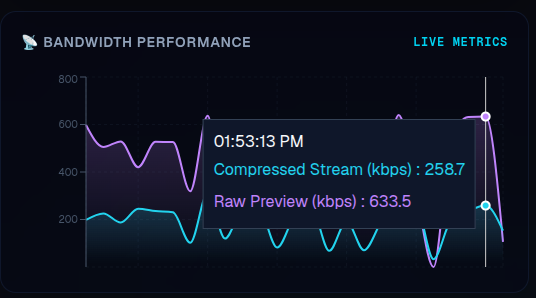
\includegraphics[width=0.44\textwidth]{Live_Bandwidth_Tracking.png}}
\hfill
\subfloat[Incident tracking and timeline\label{fig:incident_track}]{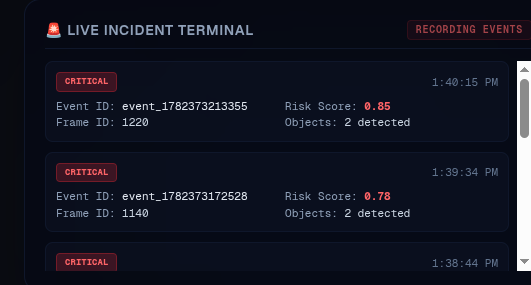
\includegraphics[width=0.44\textwidth]{Live_Incident_Tracking.png}}
\caption{Live monitoring dashboards: (a) bandwidth monitoring and savings, (b) incident tracking and timeline}
\label{fig:live_tracking}
\end{figure*}

\subsection{Operational Profiles}
Five predefined profiles enable rapid deployment: (i) Ultra Low Bandwidth (200~Kbps target; bg-scale 0.2, bg-quality 5, detect every 6 frames) for remote sites with satellite uplinks~\cite{liu2025edge}; (ii) Balanced (1~Mbps) for retail and office environments; (iii) High Quality (4~Mbps) for critical infrastructure; (iv) Privacy Mode with face and background masking for legally sensitive environments~\cite{kim2024privacy}; and (v) Custom for specialized deployments. This makes solar powered construction site cameras feasible below 200~Kbps, and enables a 50 store retail chain to centralize monitoring within 15~Mbps of ordinary business broadband~\cite{islam2024sdn}.

\subsection{Quality Metrics}
Experimental results demonstrate stable quality across presets:

\begin{table}[t]
\centering
\small
\setlength{\tabcolsep}{5pt}
\caption{Quality metrics across compression presets}
\label{tab:quality}
\begin{tabular}{lcccc}
\toprule
Preset & PSNR (dB) & SSIM & VMAF & Det.\ Accuracy \\
\midrule
High Quality & 36.2 & 0.95 & 92.4 & 98\% \\
Balanced & 33.8 & 0.91 & 87.1 & 95\% \\
Ultra Low BW & 30.1 & 0.85 & 78.5 & 88\% \\
Privacy Mode & 31.5 & 0.88 & 82.3 & 91\% \\
\bottomrule
\end{tabular}
\end{table}

\subsection{Detection Performance}
On a laptop (Linux, 2~MP WiFi camera), YOLOv8n achieves 25--45~ms inference at 22--40~FPS on CPU only and 6--12~ms at 83--166~FPS with CUDA acceleration.

\begin{table}[t]
\centering
\small
\caption{YOLOv8 nano inference performance on laptop with 2~MP WiFi camera}
\label{tab:detection}
\begin{tabular}{lcc}
\toprule
Configuration & Inference (ms) & Max FPS \\
\midrule
CPU only & 25-45 & 22-40 \\
CUDA accelerated & 6-12 & 83-166 \\
\bottomrule
\end{tabular}
\end{table}

\subsection{Audio Detection Results}
Phase 1 delivers zero false positives over 30+ minutes of silence testing with impulse detection latency $<$46~ms and a 5 second cooldown preventing echo triggers. Phase 2 provides 11 class classification with confidence threshold 0.3 and Socket.IO emission latency $<$50~ms. Audio events from critical classes with confidence $\geq$ 0.6 trigger heatmap weighting at 4.0$\times$ confidence with 2 minute spatial decay, providing persistent threat awareness.

\subsection{Activity Heatmap}
A real-time activity heatmap provides visual situational awareness:

\begin{figure}[t]
\centering
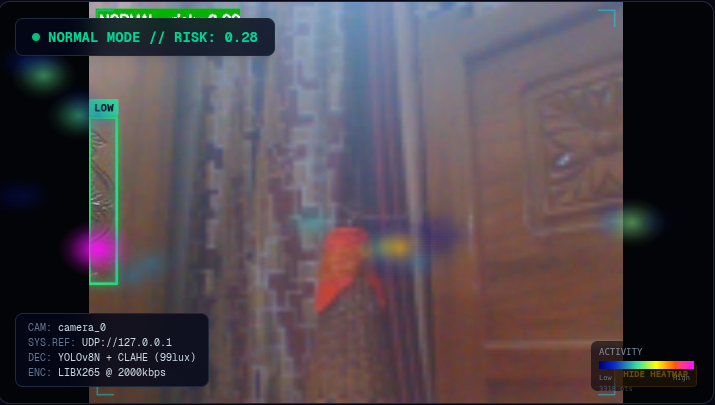
\includegraphics[width=\columnwidth]{HeatMap.png}
\caption{Activity heatmap with neon-to-cyan-to-magenta color mapping for low-light visibility, updated every 5 seconds with audio event integration}
\label{fig:heatmap}
\end{figure}

\section{Additional Subsystems}
Several substantial subsystems operate in the background. An Event Buffer and Forensics Suite keeps a rolling 15 second pre-event ring buffer of full resolution frames; when a critical event triggers, pre-event frames (225 at 15~fps) and 10 seconds of post-event frames are saved to disk with full metadata, capturing events with context rather than compressed aftermath.

A Cross Camera Re-Identification Tracker matches persons across non overlapping camera views using HSV color histograms and Local Binary Pattern texture features with cosine similarity and a 60 frame TTL track database. A PTZ Auto Tracking Controller provides ONVIF and HTTP based proportional tracking that centers high priority objects with a configurable deadzone. Docker Compose deployment orchestrates three services (edge-node, server, dashboard) with single and multi-camera profiles, enabling self configuration within 30 seconds. An experiment database archives over 814 runs across compression profiles, codecs, and environmental conditions for analysis and optimization.

\section{Related Work}
Recent ROI based compression approaches~\cite{wang2025compression,li2024region,labiod2023region,aliouat2023region} validate ROI coding benefits but are predominantly simulation based and lack real-time edge deployment with neural detection. Deep learning driven systems include DeepStream~\cite{guo2023deepstream}, achieving 54\% bandwidth reduction via adaptive frame dropping, and FRVC~\cite{agrawal2025frvc}, achieving up to 85\% storage reduction by discarding irrelevant frames in stored video; both lack per frame spatially variable compression. Rate control work~\cite{gadot2025rlrc,rozek2025video,chuang2025adaptive} focuses on rate distortion optimization rather than risk aware surveillance automation. Learned and transformer based compression~\cite{balle2017end,minnen2018joint,lu2024transformer} outperforms traditional codecs but is computationally prohibitive for cost sensitive edge deployments. Network level and privacy approaches~\cite{islam2024sdn,kim2024privacy,zhao2025federated} address infrastructure and ethical concerns but not compression efficiency directly.

Our work differs in four respects: unlike ROI-only schemes~\cite{wang2025compression,li2024region,labiod2023region} it couples real-time detection with a risk aware state machine that escalates quality during incidents; unlike frame dropping~\cite{agrawal2025frvc} it preserves every frame through spatially variable compression; unlike RL based rate control~\cite{gadot2025rlrc} its risk score is interpretable and maps directly to operational states; and unlike learned compression~\cite{lu2024transformer} it runs in real time on modest edge hardware. The combination of audio visual fusion, temporal ROI smoothing, interactive control, and evaluation across PSNR, SSIM, VMAF, and detection retention distinguishes it from existing solutions.

\section{Conclusion}
This paper presented an adaptive CCTV compression system integrating YOLOv8 based ROI control with a risk aware event engine and audio visual fusion to achieve intelligent bandwidth reduction~\cite{jocher2023yolov8,gadot2025rlrc}. The three-tier architecture spanning edge node, central server, and interactive dashboard provides a production ready surveillance platform~\cite{liu2025edge}. Experimental results demonstrate 80--95\% bandwidth reduction while maintaining stable quality (PSNR 30--36~dB, SSIM 0.85--0.95, VMAF 78--92), comparable to state of the art ROI based frameworks~\cite{wang2025compression,agrawal2025frvc}, with pre/post-event buffering preserving forensic evidence during critical incidents~\cite{chuang2025adaptive}.

The key insight is that security cameras are not televisions: they need to watch, listen, and remember, efficiently discarding hours of inactivity while capturing critical moments at maximum fidelity. Future work includes deployment on dedicated edge AI hardware, integration with cloud storage tiers, YOLOv8 segmentation for finer ROI boundaries, and multi-camera scalability validation with cross-camera re-identification at scale.

\bibliographystyle{IEEEtran}
\bibliography{references}

\end{document}
